This blocks controls its output \sig{charge} based on the voltage pulses received on its inputs \sig{start} and \sig{stop}, so that the next block \blk{rampgen} can control its output \sig{measure} based only on the current value of its inputs.

\subsection{Derivation of a Truth Table}
First, we notice that the system needs to have a memory.
Indeed, after a pulse has occured, and when both inputs are \sigval{LO}, the output \sig{charge} can still be \sigval{HI} or \sigval{LO} depending on the last pulse.
Given the logic that needs to be implemented and the fact that there are two separate pulse inputs we choose to implement the memory using an RS-latch.
This choice will prove to be adequate at the end of this section.
Intuitively, we choose to put \sig{start} on the \sig{set} of the latch and \sig{stop} on the \sig{reset}.

Furthermore, we cannot immediately reset \sig{measure} to ground upon receiving a pulse on \sig{stop}, because this would not give enough time for the output stage to properly latch the final value\footnote{In our case the output stage does not even have a memory so this does not really apply.}, or more generally, would not leave time for any reading device to use the measurement.
For this reason, we choose to reset the whole device at the rising edge of a pulse on \sig{start}, and to start the measurement at the falling edge of the pulse.
To correctly measure the delay, the measurement must then be stopped at the falling edge of the pulse on \sig{stop}.
The output voltage is thus stabilized at its final value and available for reading from the end of the \sig{stop} pulse until the beginning of the next \sig{start} pulse.

With that it mind, it is possible to derive a first logical function, where \sig{q} is the output of the RS-latch:
\begin{equation}
\sig{charge}(\sig{start}, \sig{stop}, \sig{q}) = \sig{q}\cdot\signot{start} + \sig{stop}\label{eqn:1logic}
\end{equation}

\subsection{\hspace{-.3em}\gate{nand}/\gate{nor} Implementation}
This function must be adapted based on the following implementation details:
\begin{itemize}
  \item As will be shown in next section, \sig{charge} should be active-low because it drives a PMOS switch.
  \item \gate{nand} and \gate{nor} gates are the most directly available and require less transistors than \gate{and} and \gate{or} gates.
  \item $\signot{q}$ is directly available from the RS-latch.
\end{itemize}

Using de Morgan's law on the first term of the \gate{nor} which appears when taking account that \sig{charge} should be active low, we find:
\begin{align*}
\signot{charge} &= \gate{nor}(\sig{q}\cdot\signot{start}, \sig{stop})\\
&=\gate{nor}(\gate{nor}(\signot{q}, \sig{start}), \sig{stop})
\end{align*}
This final expression allows to implement the required logic using only one RS-latch and two \gate{nor} gates (rather than for example four \gate{not}, one \gate{nand} and one \gate{nor} gate if we simply inverted function \ref{eqn:1logic}), as shown on figure~\ref{fig:blklogic}.
\begin{figure}
  \centering
  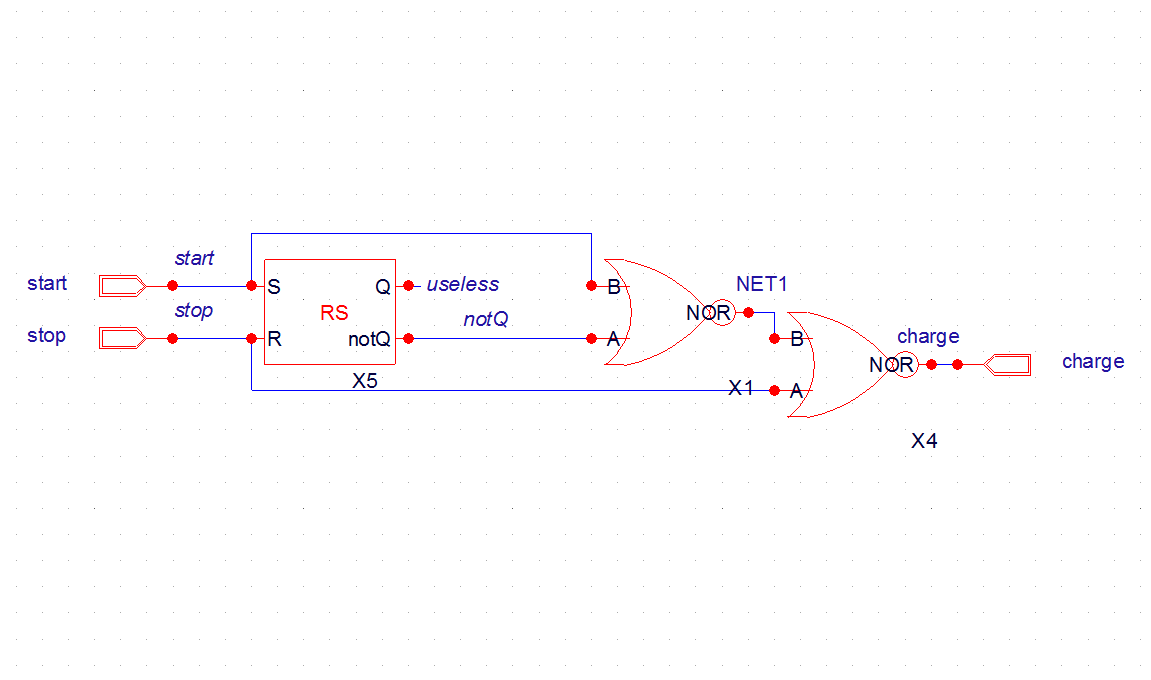
\includegraphics[width=\textwidth]{logicGates.png}
  \caption{Gate circuit of \blk{logic}.\label{fig:blklogic}}
\end{figure}

\subsection{Sizing}
The logical gates are built using minimal length transistors. The width should theoretically progressively increase from input gates to output gates so that the output gate is able to drive the parasitic input capacitance of the next block and so that every gate in the circuit is able to drive the gate at its output. However, it turns out that minimally-sized transistors are able to correctly drive \blk{rampgen}, so the whole logic circuit is made of minimally-size transistors.
